%\documentclass[fignum,letterpaper,12pt,titlepage]{article}
\documentclass[fignum,letterpaper,12pt]{article}
\usepackage[applemac]{inputenc}
\usepackage{amsfonts}
\usepackage{amsmath}
\usepackage{fullpage,array,amsmath,graphicx,psfrag,amssymb,subfigure,tabularx,booktabs}
\usepackage{amssymb}
\usepackage{graphicx}
\usepackage{rotating}
\usepackage{setspace}
\usepackage{natbib}
\usepackage[hang,small,bf]{caption}
\usepackage{subfigure}
\usepackage[toc,page]{appendix}
\usepackage{verbatim}
%\usepackage{hyperref}
\usepackage{rotating}
\usepackage{changebar}
\usepackage{pifont}
\usepackage{color}
\usepackage{endnotes}
\let\footnote=\endnote
\usepackage{dcolumn}
\clubpenalty = 10000
\widowpenalty = 10000 
\displaywidowpenalty = 10000
\usepackage[paper=letterpaper,left=20mm,right=20mm,top=25mm,bottom=25mm]{geometry}
\setlength{\parindent}{1cm}

\newcommand{\iid}{\stackrel{\mathrm{iid}}{\sim}}

\title{Beliefs about Data Quality and Implications for Inference}
\author{
Max Gallop\\
	Duke University\\
\and
Simon Weschle\\
	Duke University\\
}

\footnotesize{\date{\today}}

\graphicspath{{graphs/}}
\begin{document}
\maketitle
\thispagestyle{empty}

\section{Idea}
\noindent
Suppose we are interested in a variable $\mathbf{t}$ with elements $t_i$, where $i=1, \dots, n$. The variable is not perfectly measured and we observe $\mathbf{x}$ instead. We suspect that there is a variable $\mathbf{w}$ that systematically influences how close the elements $x_i$ are to $t_i$. Possible examples are:
\begin{itemize}
\item Historical records for the number of fatalities of wars. This series becomes potentially more accurate over time as better logistics and data processing capability makes it easier to keep track of the number of fatalities. So here $\mathbf{t}$ is the true number of fatalities, $\mathbf{x}$ the number of observed fatalities and $\mathbf{w}$ would be time.
\item A cross-national survey asking respondents e.g. whether they have bribed officials, have been the victim of police brutality, or whether they have received clientelistic benefits in exchange for vote support. One suspicion is that respondents in countries with a more repressive regime are less likely to answer ``yes'' to each of those questions.
\item The W-ICEWS data reports the monthly number of events for certain events of interest for almost all countries in the world. These events are gleaned from news stories. Since correspondents that are based in some country often also cover a number of other countries in the region, one can expect that the further countries are away from the nearest correspondent the more events will go unreported. 
\end{itemize}
The goal of the approach is to quantify \textit{beliefs} about how variable $\mathbf{w}$ systematically influences how the true values $\mathbf{t}$ are reported in $\mathbf{x}$. Given these subjective beliefs, the approach can then perform a sensitivity analysis and give information on how robust the results are to suspected systematic measurement error.


\section{Math}

\subsection{Continuous Variable}

Suppose $\mathbf{t}$ (and its realization $\mathbf{x}$) is a continuous variable with support on the real line. We model the relationship between true and observed values as follows:
\begin{equation}
t_i = x_i \cdot m_i
\end{equation} 
where $m_i$ is our \textit{belief} about how well $x_i$ measures $t_i$. If $m_i=1$ we believe that $x_i$ measures $t_i$ correctly, if $m_i<1$ we believe that $x_i$ is larger than $t_i$ and if $m_i>1$ we believe that $x_i$ is smaller than $t_i$. The value of $m_i$ is modeled as a polynomial function of $w_i$:
\begin{equation}
m_i = \alpha_0 + \sum_{j=1}^{k} \alpha_j w_i^j
\end{equation} 
where $k$ is the order of the polynomial.

\subsubsection{Example}
In this example we estimate a regression $y_i=\beta_0 + \beta_1 x_{1i} + \beta_2 x_{2i} + \beta_3 x_{4i}$, but the measurement $\mathbf{x_1}$ of $\mathbf{t_1}$ is systematically biased. Suppose the true mechanism is $t_{1i}=x_{1i} \cdot m_i$ and $m_i=1.2 + 0.05 w_i$. Further assume our beliefs about $\mathbf{m}$ are correct but we express some uncertainty. In particular, our beliefs are $\alpha_0 \sim N(1.2, 0.05)$ and  $\alpha_0 \sim N(0.05, 0.01)$. Figure \ref{beliefplot} gives the the relation between $\mathbf{w}$ on the horizontal axis and $\mathbf{m}$ on the vertical axis. The dots are the mean beliefs and the dashed lines present the area where we are 95\% confident the true value lies within. Here the belief is that $\mathbf{t_1}$ is correctly measured at low values of $\mathbf{w}$ but $\mathbf{t_1}$ is much larger than $\mathbf{x_1}$ at high values of $\mathbf{w}$ (up to almost 50\%).

\begin{figure}[h]
\begin{center}
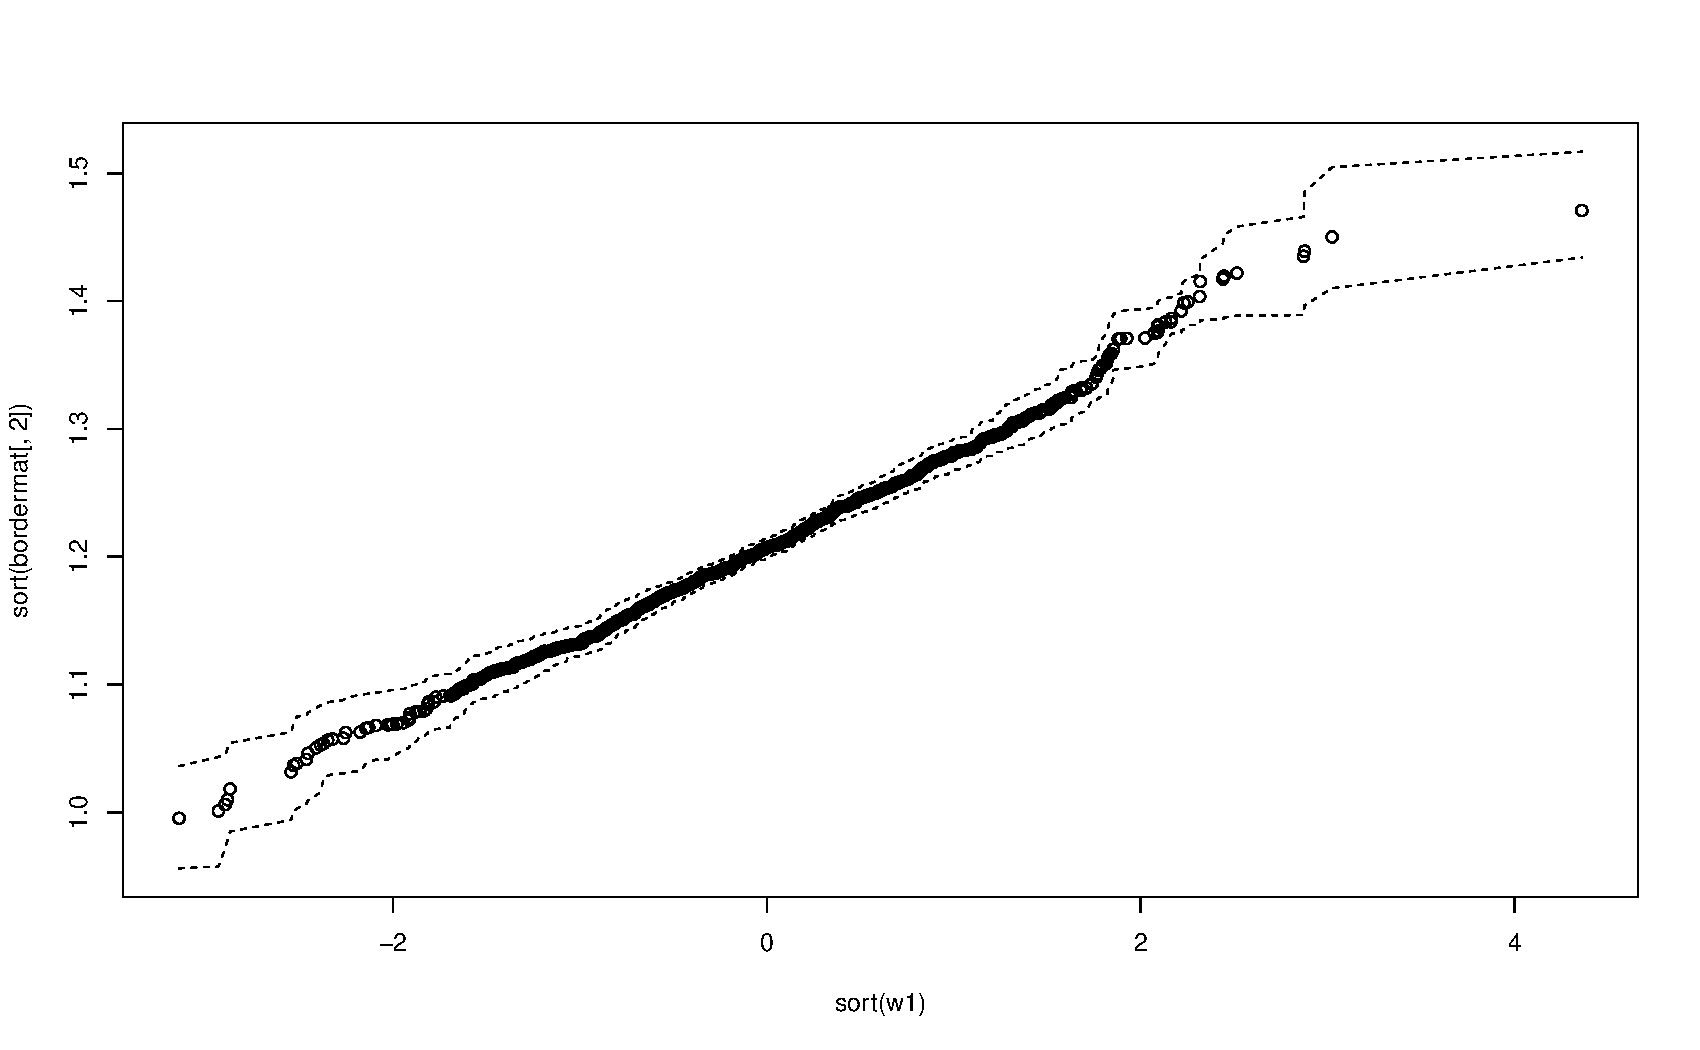
\includegraphics[width=.65\textwidth]{beliefplot.pdf} 
\caption{Description.}
\label{beliefplot}
\end{center}
\end{figure}


Figure \ref{coefplot} gives the posterior distribution of $\beta_1$, $\beta_2$ and $\beta_3$ for three different regressions. The black curves are the posteriors if we know the true values $\mathbf{t_1}$. The blue lines are what we get if we use $\mathbf{x_1}$ instead. Clearly the estimated coefficients are biased. Especially the estimated effect of the variable that is measured incorrectly on $\mathbf{y}$ is too large. The red lines give the posterior distributions after we corrected using our correct beliefs (based on 100 draws from our distribution of beliefs about $\alpha_0$ and $\alpha_1$). The posterior is relatively close to the correct posterior. 


\begin{figure}
\begin{center}
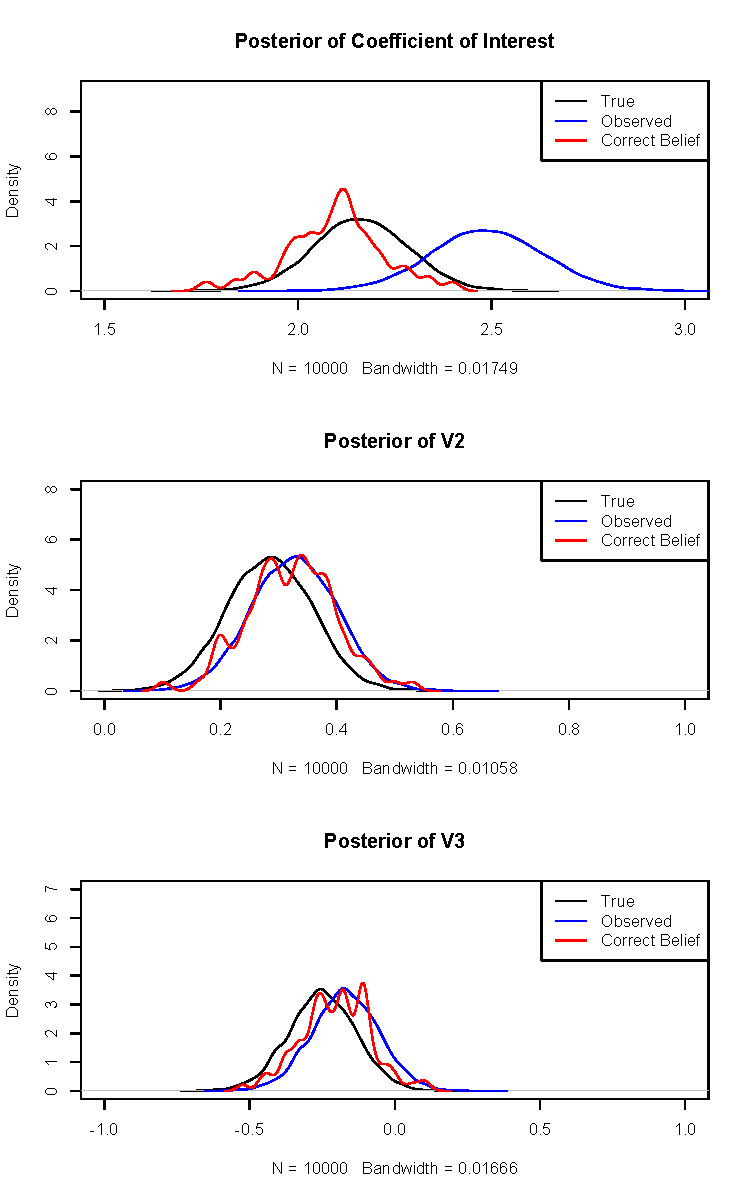
\includegraphics[width=.65\textwidth]{coefplot.pdf} 
\caption{Description.}
\label{coefplot}
\end{center}
\end{figure}



\subsection{Categorical Variable}

Suppose $\mathbf{t}$ (and its realization $\mathbf{x}$) is a categorical variable with $s$ categories.


\subsection{Binary Variable}

Suppose $\mathbf{t}$ (and its realization $\mathbf{x}$) is a binary variable.



\end{document}



